\section{TinyDAS}
\label{res:tinydas}

In this section, we'l be looking at the results for both training our autoencoders, as well as testing our models on the test data mentioned in the method section.

\subsection{Result Setup}

All the models were trained and tested on \gls{idun} computers made for \acrshort{hpc}. Configuration parameter for the different models can be found in the appendix \ref{app:judasnethyperparams}, and details of the machines used can be found in the table below. \\



\begin{table}[!h]
\centering
\begin{tabular}{|l|c|}
\hline
\textbf{Unit} & \textbf{Description}         \\ \hline
OS            & Ubuntu Linux          \\ \hline
GPU           & NVIDIA H100 HBM3     \\ \hline
VRAM          & 80GB                  \\ \hline
Gpu Cores     & 4352                  \\ \hline
Amount        & 4 (1 for testing)     \\ \hline
\end{tabular}
\label{tab:specs}
\caption{Specs for the machines running and resting the models}
\end{table}





\subsection{Experiment 1: Model training}

All models are trained using the ADAM optimizer.

\begin{table}[!htbp]
    \centering
    \begin{tabular}{lcccc}
        \hline
        \textbf{Metric} & \textbf{AE} & \textbf{CAE} & \textbf{VAE} & \textbf{CVAE} \\
        \hline
        Reconstruction Error* & 0.045 & 0.032 & 0.038 & 0.029 \\
        Latent Space Dimension Size & 64 & 128 & 64 & 128 \\
        Median time p/epoch(s) & 120 & 180 & 150 & 210 \\
        \hline
    \end{tabular}
    \caption{Comparison of Autoencoder Performance\\ *The Reconstruciton error is the sum of all reconstruction errors across all batches.}
    \label{tab:autoencoder_comparison}
\end{table}

\subsubsection{Loss Functions}

Each autoencoder type utilizes a different loss function, as outlined in Table \ref{tab:loss_functions}.

\begin{table}[!htbp]
    \centering
    \begin{tabular}{ll}
        \hline
        \textbf{Model Type} & \textbf{Loss Function} \\
        \hline
        AE & \acrshort{mse} \\
        CAE & \acrshort{mse} \\
        VAE & \acrshort{mse} + KL Divergence \\
        CVAE & \acrshort{mse} + KL Divergence \\
        \hline
    \end{tabular}
    \caption{Loss Functions for Different Autoencoder Types}
    \label{tab:loss_functions}
\end{table}

\begin{figure}[!h]
  \begin{subfigure}[t]{.5\textwidth}
    \centering
    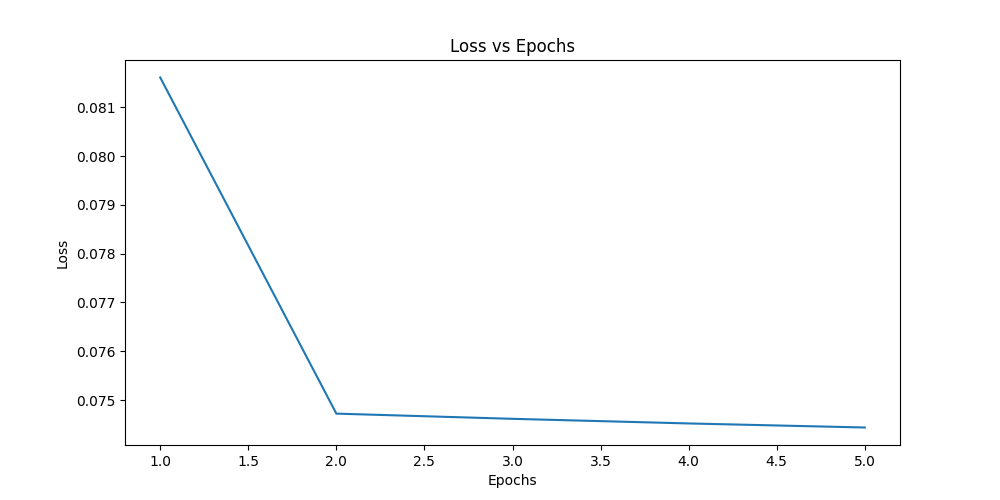
\includegraphics[width=\linewidth]{figures/loss.png}
    \caption{AE}
  \end{subfigure}
  \hfill
  \begin{subfigure}[t]{.5\textwidth}
    \centering
    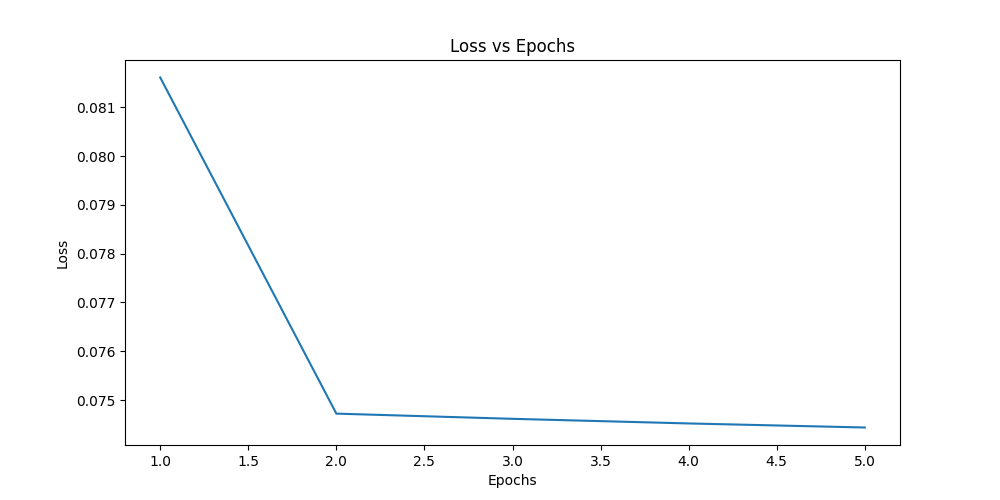
\includegraphics[width=\linewidth]{figures/loss.png}
    \caption{CAE}
  \end{subfigure}

  \medskip

  \begin{subfigure}[t]{.5\textwidth}
    \centering
    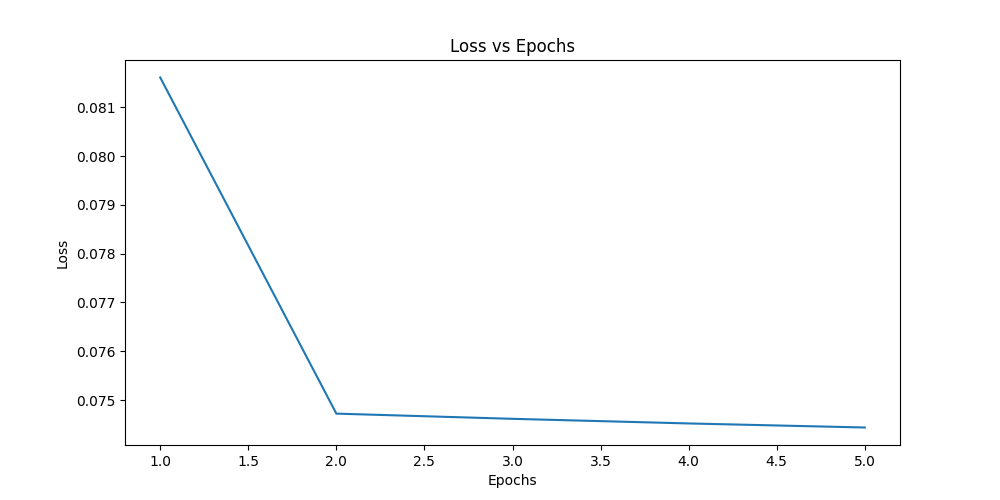
\includegraphics[width=\linewidth]{figures/loss.png}
    \caption{VAE}
  \end{subfigure}
  \hfill
  \begin{subfigure}[t]{.5\textwidth}
    \centering
    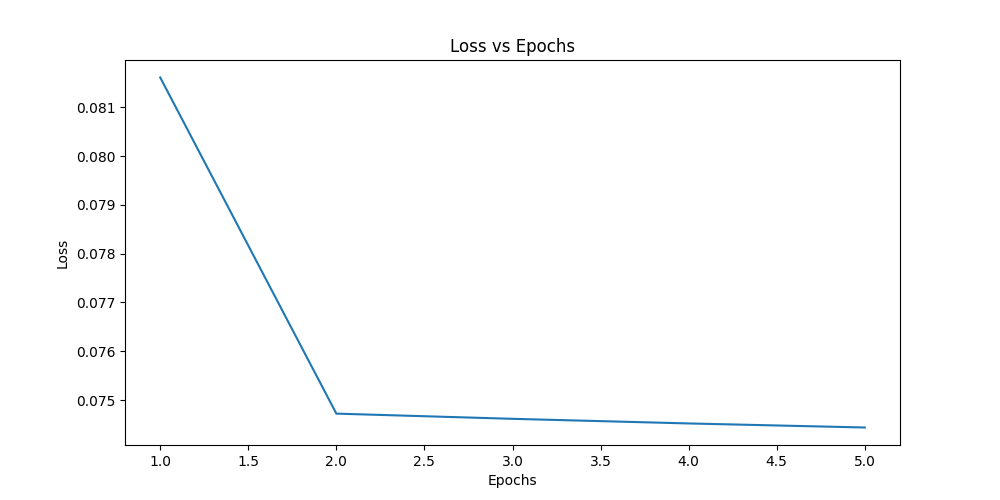
\includegraphics[width=\linewidth]{figures/loss.png}
    \caption{CVAE}
  \end{subfigure}
    \caption{Losses for all models}
\end{figure}

\subsubsection{Reconstruction Capabiltites}

\begin{figure}[!h]
    \centering
    
    % Row 0 (Image Names)
    \begin{subfigure}{0.33\textwidth}
        \centering
        \textbf{Image 1}
    \end{subfigure}%
    \hfill
    \begin{subfigure}{0.33\textwidth}
        \centering
        \textbf{Image 2}
    \end{subfigure}%
    \hfill
    \begin{subfigure}{0.33\textwidth}
        \centering
        \textbf{Image 3}
    \end{subfigure}
    
    \vspace{1em}
    
    % Row 1 (Original)
    \begin{subfigure}{0.33\textwidth}
        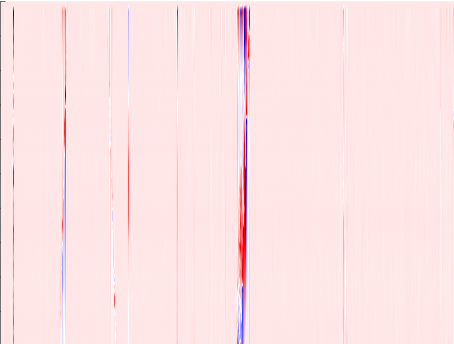
\includegraphics[width=\textwidth]{figures/test.png}
        \caption{Original}
    \end{subfigure}%
    \hfill
    \begin{subfigure}{0.33\textwidth}
        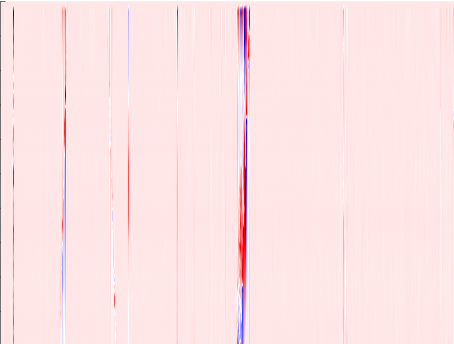
\includegraphics[width=\textwidth]{figures/test.png}
        \caption{Original}
    \end{subfigure}%
    \hfill
    \begin{subfigure}{0.33\textwidth}
        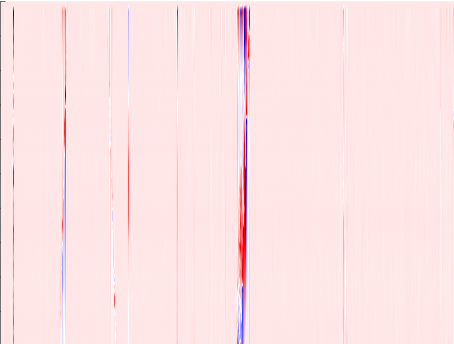
\includegraphics[width=\textwidth]{figures/test.png}
        \caption{Original}
    \end{subfigure}
    
    \vspace{1em}
    
    % Row 2 (Model 1)
    \begin{subfigure}{0.33\textwidth}
        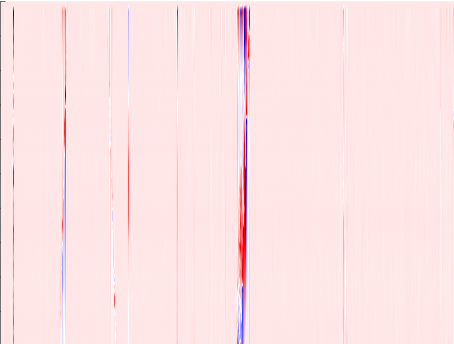
\includegraphics[width=\textwidth]{figures/test.png}
        \caption{AE}
    \end{subfigure}%
    \hfill
    \begin{subfigure}{0.33\textwidth}
        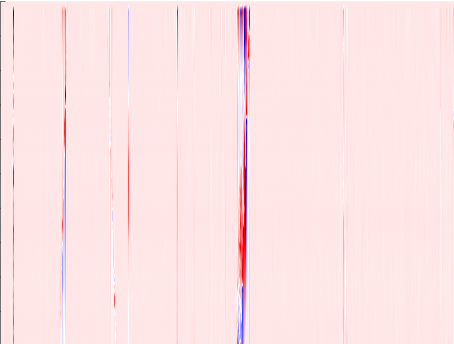
\includegraphics[width=\textwidth]{figures/test.png}
        \caption{AE}
    \end{subfigure}%
    \hfill
    \begin{subfigure}{0.33\textwidth}
        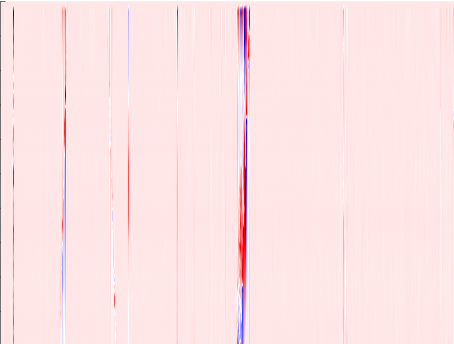
\includegraphics[width=\textwidth]{figures/test.png}
        \caption{AE}
    \end{subfigure}
    
    \vspace{1em}
    
    % Row 3 (Model 2)
    \begin{subfigure}{0.33\textwidth}
        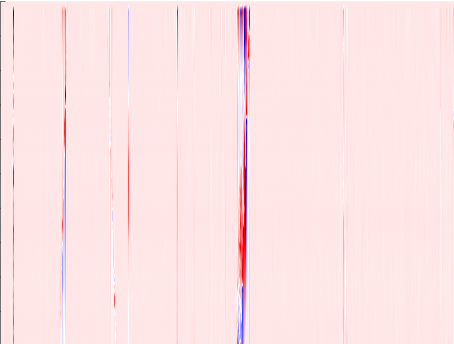
\includegraphics[width=\textwidth]{figures/test.png}
        \caption{CAE}
    \end{subfigure}%
    \hfill
    \begin{subfigure}{0.33\textwidth}
        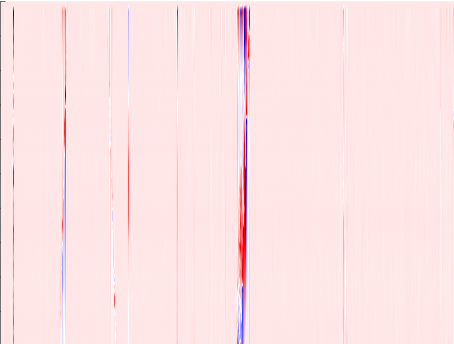
\includegraphics[width=\textwidth]{figures/test.png}
        \caption{CAE}
    \end{subfigure}%
    \hfill
    \begin{subfigure}{0.33\textwidth}
        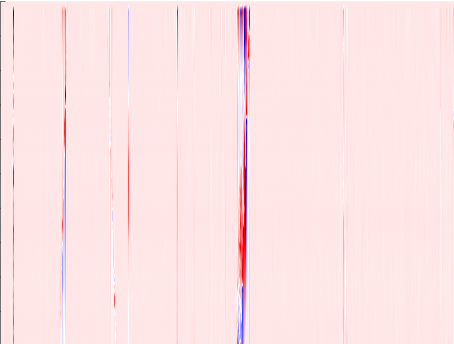
\includegraphics[width=\textwidth]{figures/test.png}
        \caption{CAE}
    \end{subfigure}
    
    \vspace{1em}
    
    % Row 4 (Model 3)
    \begin{subfigure}{0.33\textwidth}
        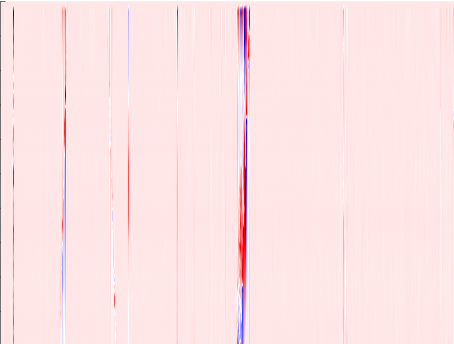
\includegraphics[width=\textwidth]{figures/test.png}
        \caption{VAE}
    \end{subfigure}%
    \hfill
    \begin{subfigure}{0.33\textwidth}
        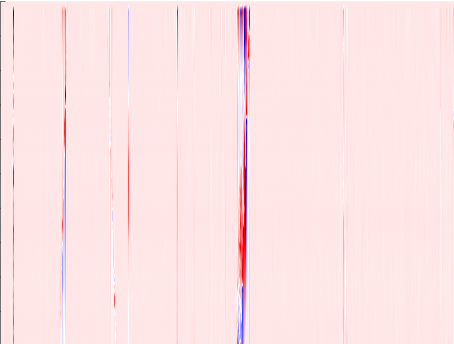
\includegraphics[width=\textwidth]{figures/test.png}
        \caption{VAE}
    \end{subfigure}%
    \hfill
    \begin{subfigure}{0.33\textwidth}
        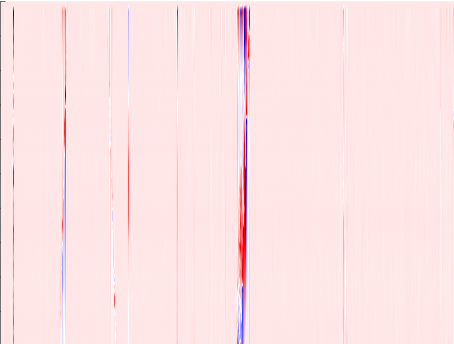
\includegraphics[width=\textwidth]{figures/test.png}
        \caption{VAE}
    \end{subfigure}
    
    \vspace{1em}
    
    % Row 5 (Model 4)
    \begin{subfigure}{0.33\textwidth}
        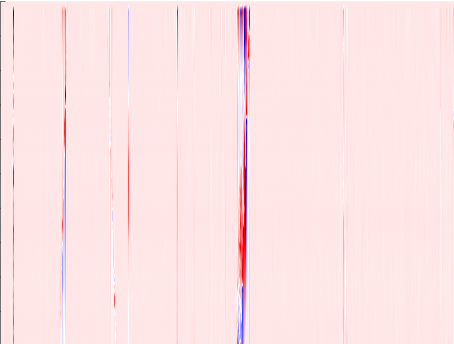
\includegraphics[width=\textwidth]{figures/test.png}
        \caption{CVAE}
    \end{subfigure}%
    \hfill
    \begin{subfigure}{0.33\textwidth}
        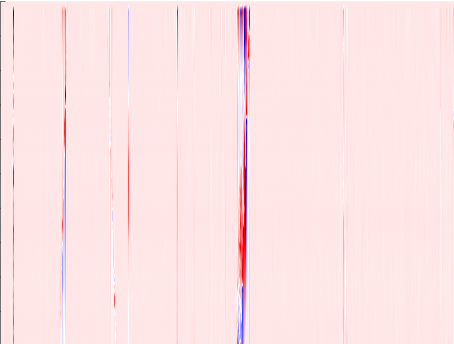
\includegraphics[width=\textwidth]{figures/test.png}
        \caption{CVAE}
    \end{subfigure}%
    \hfill
    \begin{subfigure}{0.33\textwidth}
        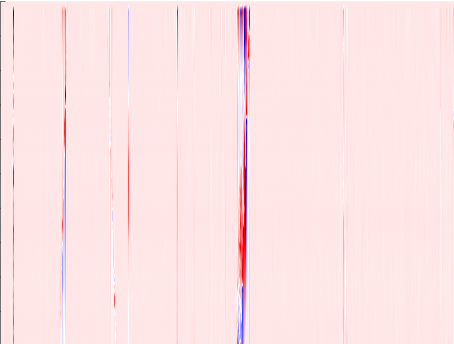
\includegraphics[width=\textwidth]{figures/test.png}
        \caption{CVAE}
    \end{subfigure}
    
    \caption{Comparison of original images and their reconstructions by different autoencoders}
    \label{fig:aereconstruct}
\end{figure}

\subsection{Autoencoder Performance Comparison}

An important part of analysing our autoencoders is the choice of metrics. Whereas loss and accuracy can provide proficient details about the model training itself, other metrics are better suited for analysing the 

Table \ref{tab:autoencoder_comparison} presents a comparative analysis of the four autoencoder types: dense, convolutional, variational dense, and variational convolutional.



\subsection{Performance Visualization}


% Confusion Matrix Components Table
\begin{table}[!h]
\centering
\begin{tabular}{l|rrrr}
\toprule
\textbf{Model} & \textbf{TP} & \textbf{FP} & \textbf{TN} & \textbf{FN} \\
\midrule
AE  & 100 & 10 & 80 & 10 \\
CAE  & 95 & 15 & 75 & 15 \\
VAE  & 105 & 8 & 85 & 5 \\
CVAE & 30 & 110 & 460 & 0 \\
\bottomrule
\end{tabular}
\caption{Confusion Matrix Components}
\end{table}

% Performance Metrics Table
\begin{table}[!h]
\centering
\begin{tabular}{l|SSSSS}
\toprule
\textbf{Model} & \textbf{TPR} & \textbf{FPR} & \textbf{Precision} & \textbf{F1-Score} & \textbf{Accuracy} \\
\midrule
AE & 0.909 & 0.111 & 0.909 & 0.909 & 0.900 \\
CAE & 0.864 & 0.167 & 0.864 & 0.864 & 0.850 \\
VAE  & 0.955 & 0.086 & 0.929 & 0.942 & 0.941 \\
CVAE & 0.91 & 0.128 & 0.91 & 0.90 & 0.817 \\
\bottomrule
\end{tabular}
\caption{Performance Metrics}
\end{table}


\begin{figure}[!h]
\centering
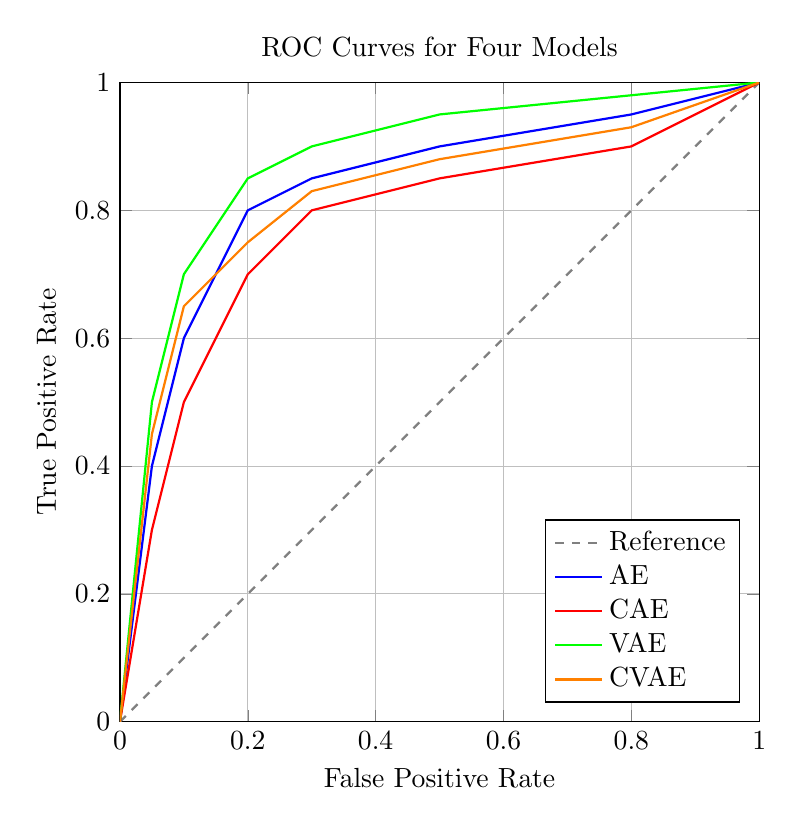
\begin{tikzpicture}
\begin{axis}[
    width=0.8\textwidth,
    height=0.8\textwidth,
    xlabel={False Positive Rate},
    ylabel={True Positive Rate},
    xmin=0, xmax=1,
    ymin=0, ymax=1,
    xtick={0,0.2,0.4,0.6,0.8,1},
    ytick={0,0.2,0.4,0.6,0.8,1},
    legend pos=south east,
    legend cell align={left},
    grid=major,
    title={ROC Curves for Four Models}
]

% Diagonal reference line
\addplot[thick,dashed,gray] coordinates {(0,0) (1,1)};

% ROC curve for Model A
\addplot[thick,blue] coordinates {
    (0,0) (0.05,0.4) (0.1,0.6) (0.2,0.8) (0.3,0.85) (0.5,0.9) (0.8,0.95) (1,1)
};

% ROC curve for Model B
\addplot[thick,red] coordinates {
    (0,0) (0.05,0.3) (0.1,0.5) (0.2,0.7) (0.3,0.8) (0.5,0.85) (0.8,0.9) (1,1)
};

% ROC curve for Model C
\addplot[thick,green] coordinates {
    (0,0) (0.05,0.5) (0.1,0.7) (0.2,0.85) (0.3,0.9) (0.5,0.95) (0.8,0.98) (1,1)
};

% ROC curve for Model D
\addplot[thick,orange] coordinates {
    (0,0) (0.05,0.45) (0.1,0.65) (0.2,0.75) (0.3,0.83) (0.5,0.88) (0.8,0.93) (1,1)
};

\legend{Reference, AE, CAE, VAE, CVAE}

\end{axis}
\end{tikzpicture}
\caption{ROC Curves Comparison for our Autoencoders }
\end{figure}

\begin{figure}[!h]
\centering
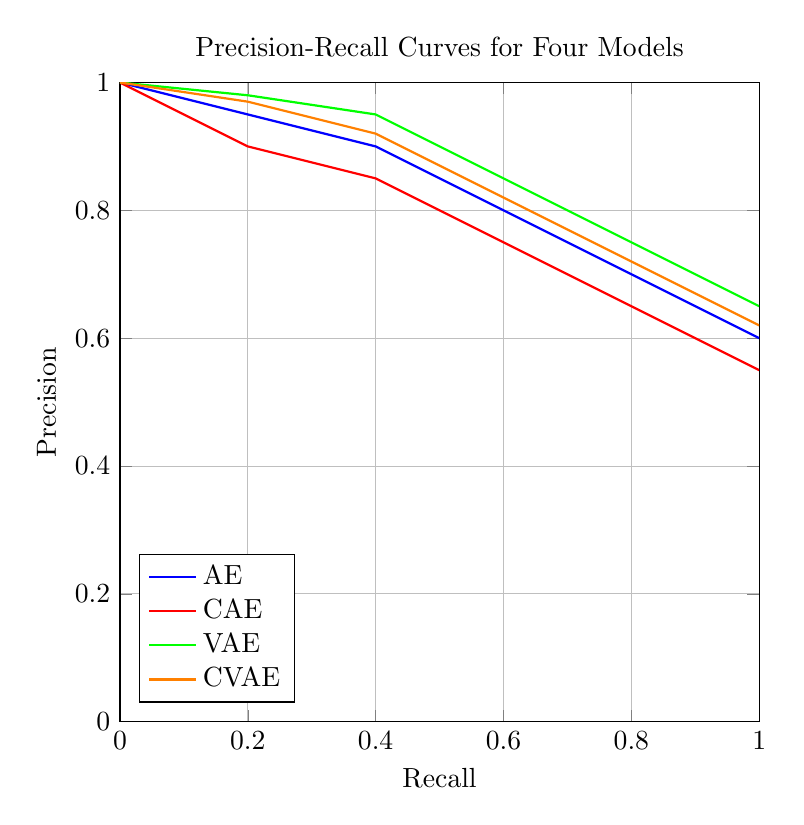
\begin{tikzpicture}
\begin{axis}[
    width=0.8\textwidth,
    height=0.8\textwidth,
    xlabel={Recall},
    ylabel={Precision},
    xmin=0, xmax=1,
    ymin=0, ymax=1,
    xtick={0,0.2,0.4,0.6,0.8,1},
    ytick={0,0.2,0.4,0.6,0.8,1},
    legend pos=south west,
    legend cell align={left},
    grid=major,
    title={Precision-Recall Curves for Four Models}
]
% PR curve for Model AE
\addplot[thick,blue] coordinates {
    (0,1) (0.2,0.95) (0.4,0.9) (0.6,0.8) (0.8,0.7) (1,0.6)
};
% PR curve for Model CAE
\addplot[thick,red] coordinates {
    (0,1) (0.2,0.9) (0.4,0.85) (0.6,0.75) (0.8,0.65) (1,0.55)
};
% PR curve for Model VAE
\addplot[thick,green] coordinates {
    (0,1) (0.2,0.98) (0.4,0.95) (0.6,0.85) (0.8,0.75) (1,0.65)
};
% PR curve for Model CVAE
\addplot[thick,orange] coordinates {
    (0,1) (0.2,0.97) (0.4,0.92) (0.6,0.82) (0.8,0.72) (1,0.62)
};
\legend{AE, CAE, VAE, CVAE}
\end{axis}
\end{tikzpicture}
\caption{Precision-Recall Curves Comparison for our Autoencoders}
\end{figure}

